%\documentclass[pageno]{jpaper}
\documentclass[conference, final]{IEEEtran}

%replace XXX with the submission number you are given from the ASPLOS submission site.
%\newcommand{\asplossubmissionnumber}{XXX}

\usepackage[normalem]{ulem}
\usepackage{tikz}
\usepackage{url}
\usepackage{pgfplots}
\usepackage{amsmath}
\usepackage{multirow}
\usepackage{enumitem}
\usepackage{listings}
\usepackage{subfig}
\usepackage{amsthm}
\usepackage[ruled,linesnumbered,lined,boxed,commentsnumbered]{algorithm2e}
\usepgfplotslibrary{statistics}


%\setlength{\textwidth}{7.5in}
%\addtolength{\oddsidemargin}{-0.2in}
%\addtolength{\evensidemargin}{-0.2in}
%\setlength{\textheight}{9.5in}
%\setlength{\topmargin}{-0.8in}
%%\setlength{\footskip}{25pt}    % page number

\definecolor{mygreen}{rgb}{0,0.6,0}
\lstset{
  frame=tb,
  tabsize=2,
  showstringspaces=false,
  language=C++,
  basicstyle=\footnotesize,
  captionpos=b,
  keywordstyle=\color{blue},
  stringstyle=\color{red},
  commentstyle=\color{mygreen},
  morecomment=[l][\color{green}]{\#}
}

%% new theory counter
\newtheorem{theorem}{Theorem}

\newcounter{theorem_counter}
\setcounter{theorem_counter}{1}


\begin{document}

\title{SimpleIdea: Colonize Jupiter with Low-cost SpaceCraft}

\author{
    Your Team Members\\
    Department of Electrical and Computer Engineering\\
    University of Utah, Salt Lake City, UT\\
}

\date{}
\maketitle

\thispagestyle{empty}

\begin{abstract}
Briefly highlight your project idea, objective, and items to achieve.
\end{abstract}

\section{Introduction}

Give a more detailed introduction about your project idea and objective.
Specifically, you will need to highlight the following items:

\begin{itemize}

\item why are you doing this? why do people care about it?
\item a set of software- and hardware-level challenges in a \textit{high-level} view
\item a set of articles you want to cite, like this nice paper~\cite{nicepaper1}

\end{itemize}

You can create a Figure \ref{fig::intro} to showcase your project.
A nice figure is more effective than saying 1000 words.

\begin{figure}[h]
  \centering
  \centerline{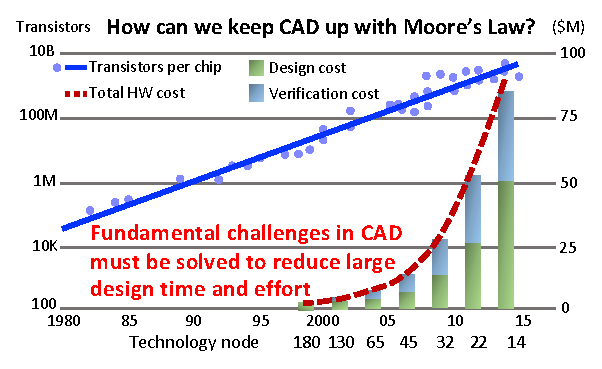
\includegraphics[width=1.\columnwidth]{Fig/intro.eps}}
  \caption{This is just a simple figure to highlight your project objective and why 
  should other people care it.}
  \label{fig::intro}
\end{figure}

\section{Challenges}

Here, go deep to your challenges at two levels, software level and hardware level.


\subsection{Software-level Challenges}

Explain the software-level challenges you encounter in your project.

\subsection{Hardware-level Challenges}

Explain the hardware-level Challenges you encounter in your project

\section{Proposed Project Execution Plan}

Go in deep how you are going to overcome the identified challenges and
write down any mitigation plan for the risks involved.

\section{Prototype}

Here, explain any preliminary results you have accomplished this semester.
This can be just a very simple prototype, but it should be something
meaningful for other people to believe in your proposed project execution plan.

\section{Team Members and Job Distributions}

List your team member names and the proposed job distributions.

\section{Timeline of Proposed Activities}

Draw a timetable or a timeline for the proposed activities 
you plan to accomplish in the next Fall semester.

\section{Availability}

List any sources, including a link to your project website,
such that people can access them.


\bibliographystyle{plain}
\bibliography{references}
%\bibliographystyle{IEEEtran}
%\bibliography{IEEEabrv,references}


\end{document}

